\documentclass[12pt]{report}
\usepackage[a4paper,top=2.5cm,right=2.5cm,bottom=2.5cm,left=2.5cm]{geometry}
\usepackage[utf8]{inputenc}
\usepackage[utf8]{vietnam}
\usepackage{multirow}
\usepackage{tikz}
\usetikzlibrary{calc}
\usepackage{fancyhdr}
\usepackage{xcolor}
\usepackage{titlesec}
\usepackage{chngcntr}
\usepackage{subcaption}
\usepackage{booktabs}
\usepackage{xurl}
\usepackage{indentfirst}
\usepackage{hyperref}
\usepackage{graphicx}
\usepackage{placeins}
\usepackage{enumitem}
\usepackage{amsmath,amsfonts,amsthm,amssymb}
\usepackage{minted}

\setlength{\headheight}{17.64015pt}
\renewcommand{\familydefault}{\sfdefault}

\pagestyle{fancy}
\setlength{\headheight}{20pt}
\lhead{}
\rhead{\leftmark}
\lfoot{}
\cfoot{\thepage}
\rfoot{}

\titleformat{\chapter}[display]{\flushright\bf\huge\color{red}}{\chaptertitlename\ \thechapter}{10pt}{}
\titleformat{\section}{\bf\Large\color{red}}{\thesection}{10pt}{}
\titleformat{\subsection}{\bf\large\color{red}}{\thesubsection}{10pt}{}
\titleformat{\subsubsection}{\bf\normalsize\color{red}}{\thesubsubsection}{10pt}{}

\newcommand{\apachejmeter}{\textbf{Apache JMeter}}
\newcommand{\jmeter}{\textbf{JMeter}}
\newcommand{\apache}{\textbf{Apache}}
\newcommand{\java}{\textbf{Java}}
\newcommand{\jmeterhome}{\texttt{\$JMETER\_HOME}}

\begin{document}

\begin{titlepage}
    \begin{tikzpicture}[remember picture, overlay]
        \draw[double,double distance=5pt,ultra thick] ($(current page.north west) + (2cm,-2cm)$) rectangle ($(current page.south east) + (-2cm,2cm)$);
    \end{tikzpicture}

    \begin{center}
        \vfill
        {\LARGE\bf Kiểm thử và đảm bảo chất lượng phần mềm} \\
        {\Large\bf INT3117 1, học kỳ II năm học 2020$-$2021} \\
        \bigskip
        \bigskip

        \bigskip
        {\Huge\bf Tìm hiểu công cụ Apache JMeter}
        \bigskip

        \bigskip
        \bigskip

        % chktex-file 44
        \begin{tabular}{c|l}
            \multirow{2}{*}{Thành viên nhóm} & Ngô Quang Dương (17020191)    \\
                                             & Nguyễn Phương Hiếu (17020747) \\
        \end{tabular} \\
        \medskip
        {\today}
        \vfill
    \end{center}
\end{titlepage}

\tableofcontents

\chapter{Giới thiệu}

\section{Lịch sử}

\par \jmeter{} là một dự án mã nguồn mở của \apache{}, được viết hoàn toàn bằng \java{}. \jmeter{} cung cấp giao diện đồ họa sử dụng Swing. Mã nguồn của dự án được public trên GitHub:~\url{https://github.com/apache/jmeter}

\par \jmeter{} được sử dụng để kiểm tra hiệu năng của server (web server, FTP server, mail server, \ldots), giả lập lượt truy cập, hiển thị kết quả kiểm tra hiệu năng trên giao diện đồ họa.

\par Người đầu tiên phát triển \jmeter{} là \href{https://www.linkedin.com/in/stefanom}{Stefano Mazzocchi}. Ban đầu, anh tạo ra công cụ này để kiểm tra hiệu năng cho một dự án web server là \textbf{Apache JServ}, dự án mà sau này được thay thế bằng \textbf{Apache Tomcat}. Phiên bản 1.0 của \jmeter{} được đưa ra vào cuối năm 1998. Từ đó đến nay, các tính năng của \jmeter{} liên tục được bổ sung và nâng cao.

\par Ban đầu, \jmeter{} chỉ được thiết kế để kiểm tra hiệu năng của các ứng dụng web. Về sau, \jmeter{} được cung cấp thêm các tính năng khác cho việc kiểm thử chức năng và hiệu năng.

\section{Cài đặt}

\par Ở thời điểm báo cáo này được viết, phiên bản mới nhất của \jmeter{} là 5.4.1. \jmeter{} có thể được tải về dưới một trong hai dạng: \textit{mã nguồn} và \textit{binaries} từ website
\begin{quotation}
    \url{https://jmeter.apache.org/download_jmeter.cgi}
\end{quotation}

\par Phiên bản này yêu cầu máy có \java{} 8+. Nếu chọn cách tải mã nguồn, máy cần được cài thêm Gradle để biên dịch.
\bigskip
\par Các phiên bản trước của \jmeter{} có thể được tải về từ link lưu trữ
\begin{quotation}
    \url{https://archive.apache.org/dist/jmeter/binaries/}
\end{quotation}

\bigskip
\par Đối với lựa chọn tải binaries, sau khi tải về và giải nén, ta có được một cấu trúc thư mục như sau:

\begin{verbatim}
bin/
  - examples/
  - report-template/
  - templates/
docs/
  - api/
  - css/
  - images/
extras/
lib/
  - ext/
  - junit/
licenses/
printable_docs/
  - demos/
  - extending/
  - localising/
  - usermanual/
\end{verbatim}

\par Trong các thư mục trên, cần lưu ý nhất tới \texttt{bin/} và \texttt{lib/}. \textbf{Quy ước trong toàn bộ báo cáo này, \jmeterhome{} là thư mục chứa \texttt{bin/} và \texttt{lib/}}.

\begin{itemize}[itemsep=0pt]
    \item \texttt{bin/} chứa các file thực thi để sử dụng \jmeter{}.
    \item \texttt{lib/}
          \begin{itemize}[itemsep=0pt]
              \item \texttt{./} các file JAR tiện ích.
              \item \texttt{ext/} các plugins cho \jmeter{}.
          \end{itemize}
\end{itemize}

\par Những file JAR của JDBC, JMS (Java Message Service, chẳng hạn như Apache Kafka) và những thư viện mà \jmeter{} cần đều được đặt trong thư mục \texttt{lib/} (không phải thư mục \texttt{lib/ext/}).

\par Để bắt đầu sử dụng \jmeter{}, truy cập thư mục \texttt{bin/} (từ Powershell/Command Prompt nếu sử dụng Windows, từ Terminal nếu sử dụng Linux/Mac), sau đó
\begin{itemize}[itemsep=0pt]
    \item Chạy file \texttt{jmeter.bat} nếu máy sử dụng Windows.
    \item Ngược lại, chạy file \texttt{jmeter}.
\end{itemize}

\par Sau đó, giao diện đồ họa của \jmeter{} hiện lên như sau:

\FloatBarrier{}
\begin{figure}[htp]
    \centering
    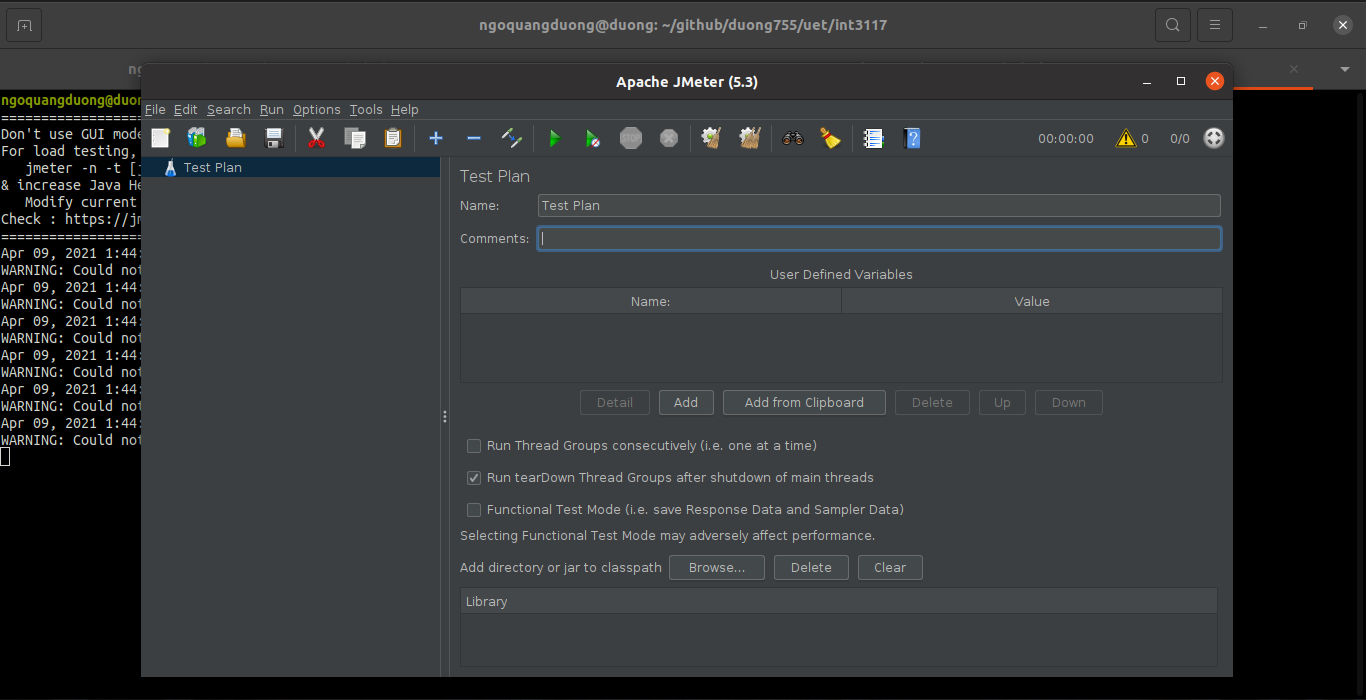
\includegraphics[scale=0.3]{jmeter_gui.png}
    \caption{Giao diện đồ họa của \jmeter{}}
\end{figure}
\FloatBarrier{}

\par Có thể có lỗi khi chạy \jmeter{} trên Linux, như việc không tìm thấy một class, chẳng hạn
\begin{quotation}
    \texttt{org.GNOME.Accessibility.AtkWrapper}
\end{quotation}

\par Để khắc phục điều này, hãy comment lại các class trong file
\begin{quotation}
    \texttt{/etc/java-8-openjdk/accessibility.properties}
\end{quotation}
\par và khởi động lại \jmeter{}.


\chapter{Một số tính năng}

\section{Kiểm tra hiệu năng}

\par Đây là tính năng chính của \jmeter{}. \jmeter{} có thể kiểm tra hiệu năng của các web server, giao thức, tiến trình khác nhau.

\par \jmeter{} có khả năng kiểm tra rộng đến vậy vì được viết hoàn toàn bằng \textbf{Java}. Công cụ này cung cấp tính năng giả lập luồng sử dụng/người dùng để test hiệu năng của hệ thống khi có nhiều lượt truy cập cùng lúc. Một lần nữa, điều này khả thi nhờ khả năng lập trình đa luồng và khả năng chịu tải ghê gớm của \textbf{Java}.

\bigskip

\par \jmeter{} có thể kiểm tra hiệu năng web server $-$ web server có thể sử dụng bất kỳ ngôn ngữ nào (vì HTTP/HTTPS độc lập với ngôn ngữ).
\par \jmeter{} kiểm tra được loại webservices như SOAP, REST, và cả GraphQL.\@
\par \jmeter{} có thể kiểm thử các kết nối, truy vấn đến các cơ sở dữ liệu thông qua JDBC.\@
\par \jmeter{} có thể kiểm tra hiệu năng của các Message-oriented Middleware thông qua Java Message Service.
\par \jmeter{} tạo được các request trên các giao thức FTP, SMTP/SMTPS, POP3/POP3S, TCP.\@

\section{Tạo báo cáo}

\par Các response, thời gian response, kết quả kiểm thử, \ldots của một \textbf{Test Plan} có thể được visualize dưới dạng biểu đồ (xem hình~\ref{fig:aggregate} và~\ref{fig:time-response}), kết xuất thành file hoặc bảng.

\begin{figure}[htp]
    \centering
    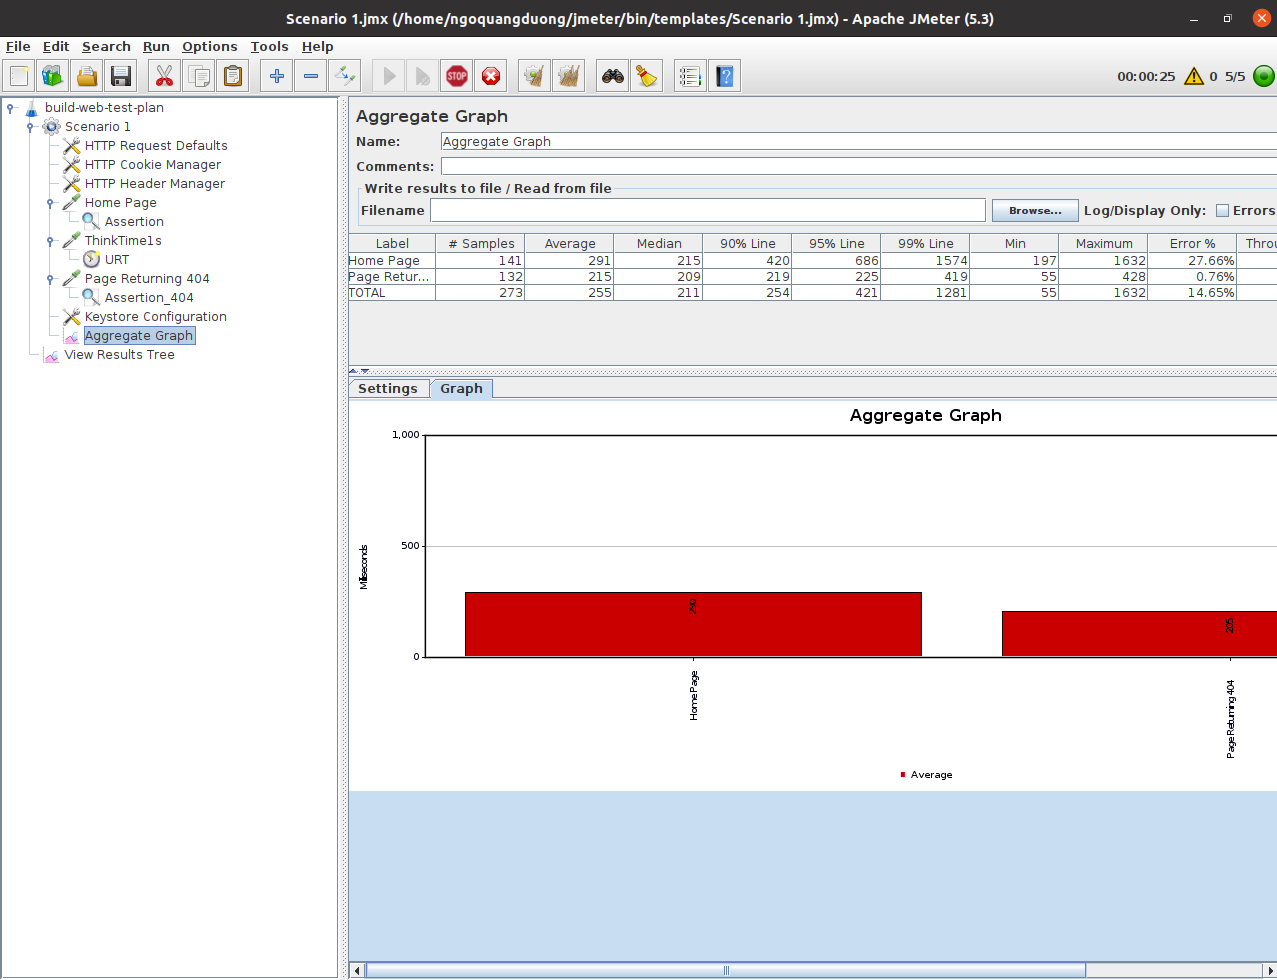
\includegraphics[scale=0.3]{aggregate.png}
    \caption{Aggregate Graph}
    {\label{fig:aggregate}}
\end{figure}

\begin{figure}[htp]
    \centering
    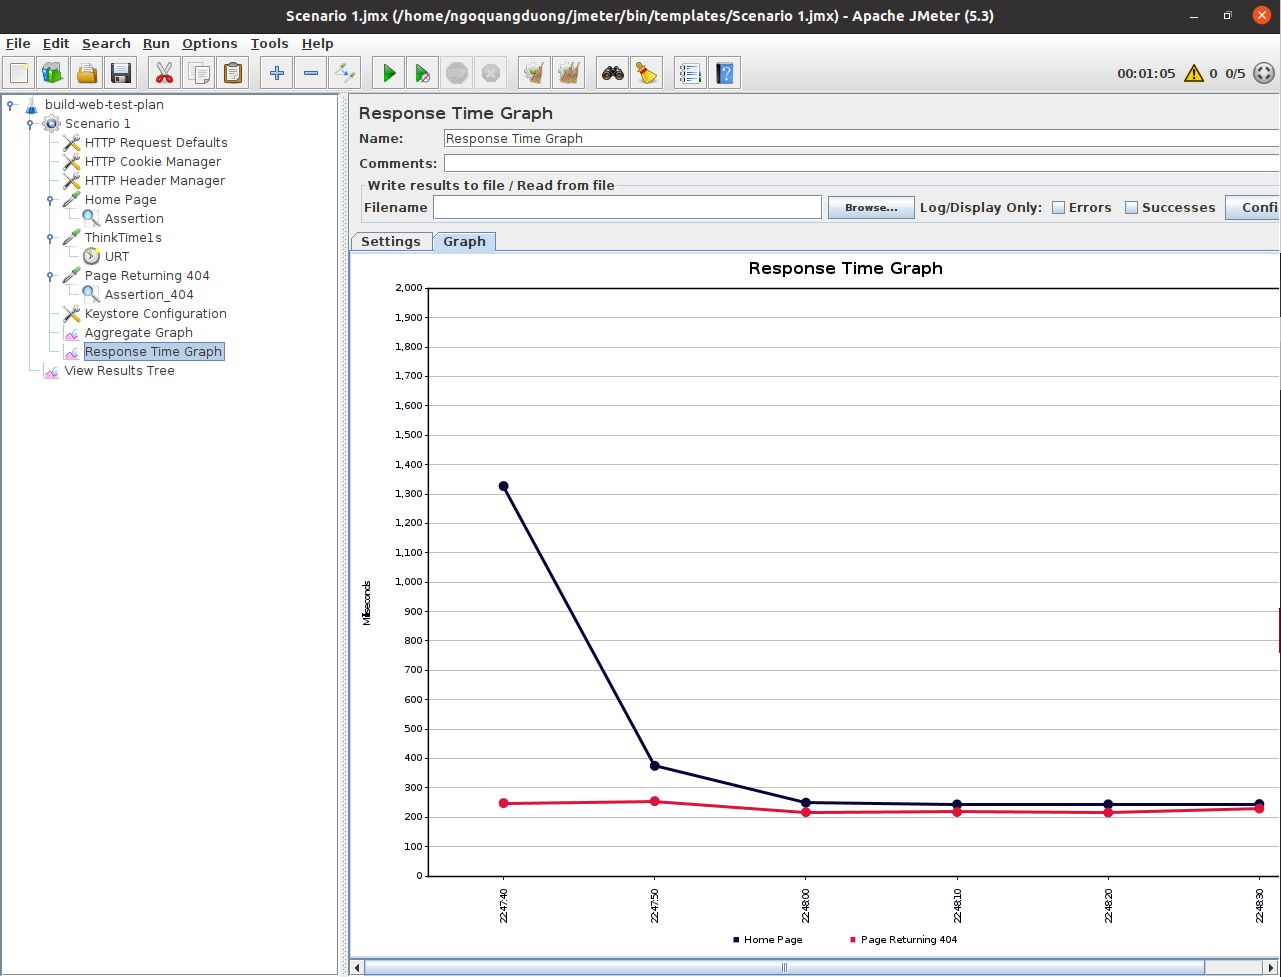
\includegraphics[scale=0.3]{timeresponse.png}
    \caption{Time Response}
    {\label{fig:time-response}}
\end{figure}

\section{Mở rộng}

\par Khả năng mở rộng của \jmeter{} đến từ hai việc:

\begin{itemize}
    \item \jmeter{} có thể được cài thêm plugins.
    \item \jmeter{} có thể tích hợp với các công cụ kiểm thử khác để thực hiện những việc mà một mình \jmeter{} không thể. \jmeter{} có thể được tích hợp với \textbf{Katalon Studio}, \textbf{Selenium IDE}.
\end{itemize}

\chapter{Các thành phần chính và cách hoạt động của JMeter}

\section{Dùng thử}

\par Trước khi trình bày về các thành phần chính và cách hoạt động của \jmeter{}, ta nên dùng thử và có cái nhìn sơ qua về một số thành phần cần lưu ý khi sử dụng công cụ này.

\par Mở \textbf{Terminal}, di chuyển đến thư mục cài đặt của \jmeter{}, chạy lệnh sau để mở giao diện đồ họa:
\begin{quotation}
    \begin{minted}{shell}
# Linux
./bin/jmeter
\end{minted}
    \begin{minted}{powershell}
# Windows
.\bin\jmeter.bat
\end{minted}
\end{quotation}

\par Để dễ dàng bắt đầu, \jmeter{} có cung cấp cho một số template.

\par Trên thanh công cụ, lần lượt chọn \texttt{File > Templates\ldots} và chọn \texttt{Building a Web Test Plan}. Workspace của \jmeter{} hiển thị lại như hình~\ref{fig:template}.

\FloatBarrier{}
\begin{figure}[htp]
    \centering
    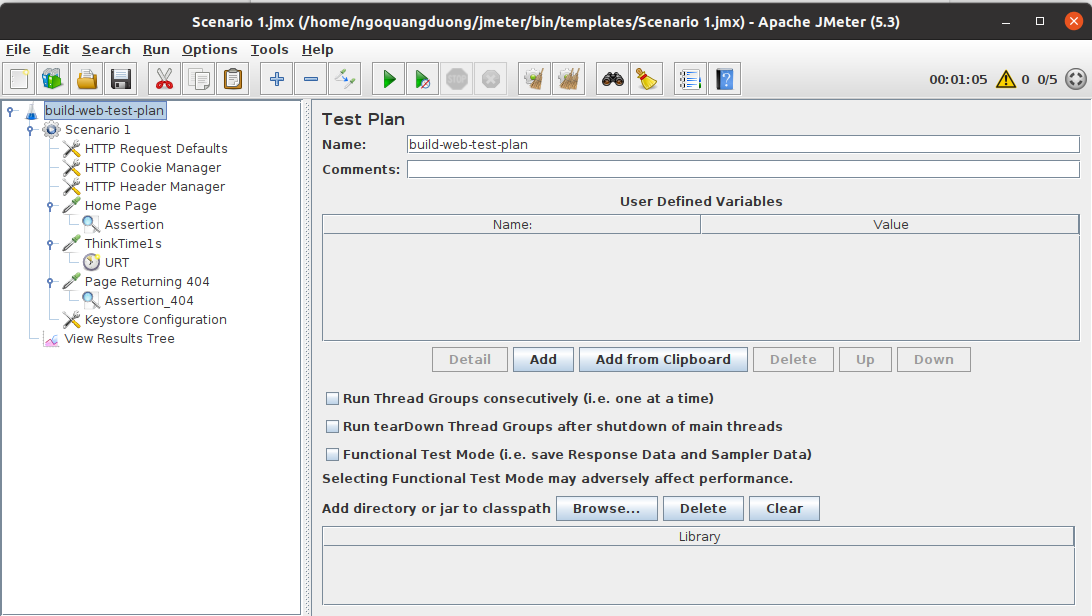
\includegraphics[scale=0.33]{template.png}
    \caption{Template}
    {\label{fig:template}}
\end{figure}
\FloatBarrier{}

\par Giải thích các thành phần trong cấu trúc cây ở bên trái của hình~\ref{fig:template}:

\begin{itemize}
    \item \texttt{build-web-test-plan}: tên của \textbf{Test Plan} (thành phần lớn nhất của \jmeter{}, mọi thứ khác đều thuộc một \textbf{Test Plan}).
    \item \textit{Scope}: Các thành phần \texttt{HTTP Request Defaults}, \texttt{HTTP Cookie Manager}, \texttt{HTTP Header Manager}, \texttt{Home Page}, \texttt{ThinkTime1s}, \texttt{Page Returning 404}, \texttt{Keystore Configuration} thuộc cùng một scope. \texttt{Assertion}, \texttt{URT}, \texttt{Assertion\_404} không thuộc scope đó.
    \item \texttt{Scenario 1}: tên của \textbf{Thread Group} (thành phần xử lý của một \textbf{Test Plan}).
    \item \texttt{Home Page, ThinkTime1s, Page Returning 404}: các HTTP request samplers, mỗi sampler sẽ thực hiện một HTTP request.
    \item \texttt{HTTP Request Defaults}: request mặc định nếu các HTTP request sampler không chỉ định Server Name hay IP.\@
    \item \texttt{HTTP Cookie Manager}: thêm cookie cho các HTTP request cùng scope.
    \item \texttt{HTTP Header Manager}: thêm header cho các HTTP request cùng scope.
    \item \texttt{Assertion}: kiểm tra response của \texttt{Home Page}.
    \item \texttt{URT}: delay \texttt{ThinkTime1s} trong 1 giây.
    \item \texttt{Assertion\_404}: kiểm tra response của \texttt{Page Returning 404}.
    \item \texttt{View Results Tree}: hiển thị các kết quả, các response của các samplers trên.
\end{itemize}

\par Để thực thi \textbf{Test Plan}, bấm nút Play. Nội dung các request/response được lưu lại trong \texttt{View Results Tree}. Khi chạy, \textbf{Test Plan} sẽ thực thi tuần tự các \textbf{samplers}.

\section{Test plan}

\par Để thực hiện việc kiểm thử với \jmeter{}, việc đầu tiên cần làm chính là tạo một Test plan.

\par Test plan chính là đơn vị/thành phần lớn nhất mà ta sẽ làm việc cùng khi sử dụng \jmeter{}. Test plan chứa một chuỗi các hành động mà \jmeter{} sẽ thực thi khi chạy test plan đó.

\par Một test plan hoàn chỉnh trong \jmeter{} bao gồm những thành phần sau:
\begin{itemize}[itemsep=0pt]
    \item Thread group.
    \item Controller.
    \item Listener.
    \item Timer.
    \item Assertion.
    \item Cấu hình.
\end{itemize}

\par Một test plan được lưu trong một file XML với phần mở rộng là \texttt{jmx}. Nội dung/thành phần của một test plan có thể được thêm/bớt/chỉnh sửa trên giao diện đồ họa của \jmeter{} hoặc thông qua việc chỉnh sửa file \texttt{*.jmx}.

\section{Thread group}

\par Thread group là thành phần bắt buộc phải có trong một test plan, đồng thời cũng là thành phần đầu tiên hoạt động khi một test plan được thực thi.

\par Thread group quản lý các luồng mà \jmeter{} sẽ sử dụng để thực hiện kiểm thử. Các luồng mà thread group quản lý được coi là sự giả lập người dùng/request, các luồng này hoàn toàn độc lập với nhau.

\FloatBarrier{}
\begin{figure}[htp]
    \centering
    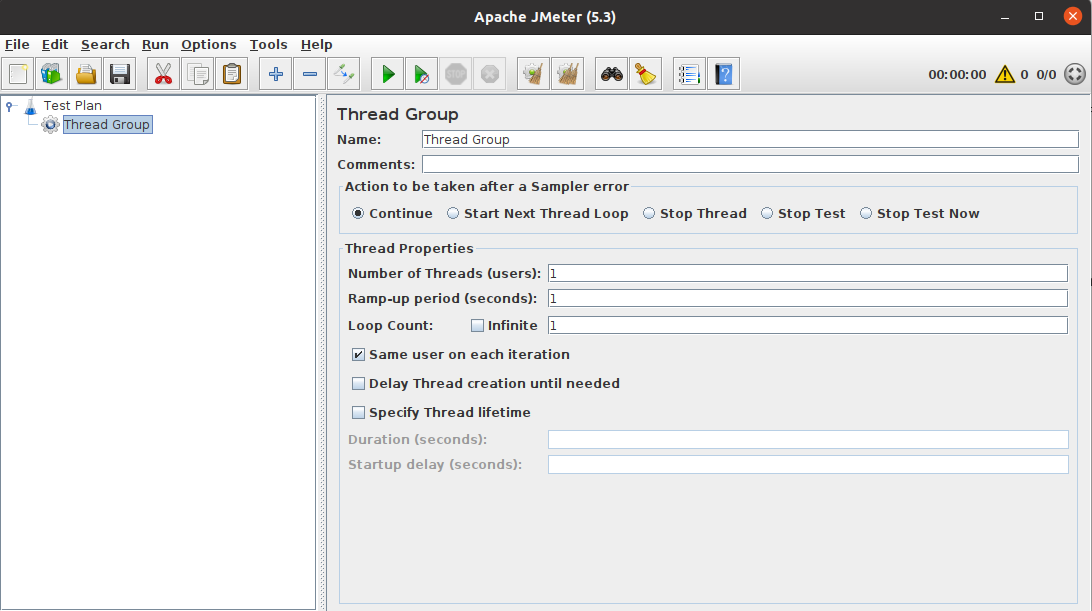
\includegraphics[scale=0.3]{thread_group.png}
    \caption{Các thuộc tính của một thread group}
    {\label{fig:thread-group}}
\end{figure}
\FloatBarrier{}

\par Như trong hình~\ref{fig:thread-group}, một thread group có các thuộc tính sau:
\begin{itemize}
    \item Number of threads ($n$): Đây là số lượng luồng mà \jmeter{} sẽ tạo và thực thi khi chạy.
    \item Ramp-up period ($t$): Thời lượng mà \jmeter{} dùng để khởi động toàn bộ số lượng luồng đã chỉ định. Chẳng hạn, nếu có $n$ luồng được tạo, còn ramp-up period là $t$ giây thì mỗi luồng sẽ bắt đầu $t/n$ giây sau khi luồng trước đó đã bắt đầu. Với cơ chế như vậy, nếu số lượng luồng là rất lớn thì ramp-up period cũng cần phải đủ lớn để tránh quá tải.
    \item Loop count ($\ell$): Sau mỗi $n/t$ giây, $\ell$ luồng sẽ chạy.
\end{itemize}

\par Ngoài ra, \jmeter{} cho phép chọn thời gian sống (duration), thời gian trễ khởi động (startup delay) của một luồng.

\section{Controller}

\par Trong \jmeter{}, controller là thành phần quyết định quá trình xử lý của một test plan, và có hai loại controller như dưới đây.

\subsection{Sampler}

\par Sampler yêu cầu \jmeter{} gửi request đến server. Chẳng hạn, để \jmeter{} gửi một HTTP request, ta cần một HTTP request sampler. Nói chung, với các giao thức/ứng dụng/dịch vụ khác nhau, có một sampler tương ứng để tạo request với giao thức/ứng dụng/dịch vụ đó.

\par Mục đích của việc sử dụng \jmeter{} là kiểm tra hiệu năng của giao thức/ứng dụng/dịch vụ $-$ do đó việc tạo request là điều phải xảy ra khi thực thi một test plan. Nói cách khác, trong một test plan, phải có ít nhất một sampler.

\par Dưới đây liệt kê một số sampler (còn có các sampler khác) có trong \jmeter{}:

\begin{itemize}[itemsep=0pt]
    \item \textbf{HTTP request}
          \par Sampler này cho phép gửi HTTP/HTTPS request đến server, thiết lập các thuộc tính của một request như method, parameter, body, file (upload) \ldots
          \par Một HTTP request sampler có thể gửi request đến một SOAP, REST web service. Hơn thế nữa, sampler này còn cho phép gửi GraphQL HTTP request.
    \item \textbf{JDBC request}
          \par JDBC request sampler gửi truy vấn SQL đến một cơ sở dữ liệu. Cần cung cấp Driver class và cấu hình JDBC để sử dụng sampler này.
    \item \textbf{Java object request}
          \par Sampler này cho phép điều khiển một class được implement interface

          \begin{quotation}
              \texttt{org.apache.jmeter.protocol.java.sampler.JavaSamplerClient}
          \end{quotation}
    \item \textbf{JUnit request}
          \par Với sampler này, \jmeter{} có thể chạy các JUnit test. Để làm được điều này, ta thực hiện các việc sau:
          \begin{enumerate}[itemsep=0pt,itemindent=1cm,label = Bước \arabic*.]
              \item Biên dịch các file chứa các test case thành những file \texttt{*.jar}
              \item Đặt các file \texttt{*.jar} vừa biên dịch vào thư mục \texttt{\jmeterhome{}/lib/junit/}
              \item Thêm JUnit request sampler vào test plan. JUnit request sampler sẽ nhận ra các class JUnit test và các method được gắn annotate \texttt{@Test}.
          \end{enumerate}
          \par Ở thời điểm viết báo cáo này, \jmeter{} chưa chính thức hỗ trợ Junit 5, mà chỉ đến JUnit 3 và 4.
    \item \textbf{Mail request}
          \par Mail request có thể được chia làm hai loại: đọc mail và gửi mail.
          \par Sampler để đọc mail là \textit{Mail Reader Sampler}. Sampler này có thể sử dụng giao thức POP3 (S) hoặc IMAP (S).
          \par Sampler để gửi mail là \textit{SMTP Sampler}. Sampler này sử dụng giao thức SMTP (S).
    \item \textbf{OS process request}
          \par Sampler này được dùng để thực thi các lệnh trên máy cài \jmeter{}. Sampler này sử dụng được trên cả Windows, Linux và Mac, mặc dù cơ chế phân tích cú pháp lệnh trên shell của các hệ điều hành này khác nhau.
\end{itemize}

\subsection{Logic controller}

\par Khác với sampler, một logic controller là thành phần không bắt buộc có trong một test plan. Nhưng logic controller quyết định thứ tự xử lý của các sampler. Logic controller chứa các sampler và còn có thể chứa các logic controller khác.

\par Dưới đây là một số controller đại diện trong \jmeter{}, tên gọi của những controller này đã cho thấy chúng hoạt động thế nào:

\begin{itemize}[itemsep=0pt]
    \item \textbf{Simple controller}
          \par Chức năng duy nhất của \textbf{Simple controller} lưu lại kết quả chạy của test plan vào một file của thư mục hiện tại (thư mục mà ở đó khởi động \jmeter{}).
    \item \textbf{Loop controller}
          \par Như tên gọi, controller này sẽ lặp lại các request.
          \par Thuộc tính duy nhất của loop controller là loop count. Thuộc tính này kết hợp với loop count của thread group $-$ tức là khi thực thi test plan, trong test plan này có một loop controller, số request được gửi sẽ là
          \[
              \text{number of requests} = \text{loop count of thread group} \times \text{loop count of loop controller}
          \]
    \item \textbf{Once only controller}
          \par Controller này chỉ cho phép request bên trong nó chạy một lần.
    \item \textbf{While controller}
          \par Controller này cần được cung cấp thuộc tính \texttt{Condition} $-$ đây là một giá trị boolean hoặc một biểu thức sẽ trả về giá trị boolean. Giá trị/biểu thức được cung cấp cho \texttt{Condition} có thể sử dụng biến và hàm của \jmeter{}.
          \par Khi chạy test plan, các thành phần của \textbf{While controller} sẽ chạy đến khi \texttt{Condition} có giá trị \texttt{false}.
          \par Nếu \texttt{Condition} bị bỏ trống hoặc có giá trị \texttt{LAST}, vòng lặp sẽ dừng lại khi sample cuối cùng trong \texttt{While controller} fail.
    \item \textbf{ForEach controller}
          \par \textbf{ForEach controller} duyệt qua một tập hợp các biến. Các biến này có cùng \textit{prefix} và được theo sau bởi số thứ tự (bắt đầu từ 1). Ví dụ:
          \begin{quotation}
              \texttt{inputVar\_1}, \texttt{inputVar\_2}, \texttt{inputVar\_3}, \texttt{inputVar\_4}
          \end{quotation}
          \par Nếu biến có giá trị \texttt{null}, sampler trong \textbf{ForEach Controller} sẽ không chạy.
          \par Mỗi lần duyệt, các sampler trong \textbf{ForEach controller} chạy thêm một lần.
    \item \textbf{If controller}
          \par Controller này cũng có một thuộc tính \texttt{Condition}, tuy nhiên giá trị/biểu thức được cung cấp cho thuộc tính này được tính toán bằng \textbf{JavaScript}.
          \par Nếu \texttt{Condition} \texttt{true}, các thành phần trong \textbf{If controller} sẽ chạy. Ngược lại, chúng sẽ bị bỏ qua.
    \item \textbf{Runtime controller}
          \par \textbf{Runtime controller} kiểm soát thời gian chạy của các thành phần bên trong nó. Thuộc tính quy định điều này là \texttt{Runtime} (tính bằng giây). Đến khi thời gian đã chạy của các thành phần trong \textbf{Runtime controller} vượt quá giá trị của \texttt{Runtime} (giây), chúng sẽ dừng lại.
    \item \textbf{Interleave controller}
          \par Trong mỗi lần duyệt (loop iteration), các sampler bên trong \textbf{Interleave controller} sẽ chạy luân phiên với các sampler cùng scope với \textbf{Interleave controller}.
          \par Cụ thể hơn, hãy theo dõi hình~\ref{fig:interleave-controller}.
          \FloatBarrier{}
          \begin{figure}[htp]
              \centering
              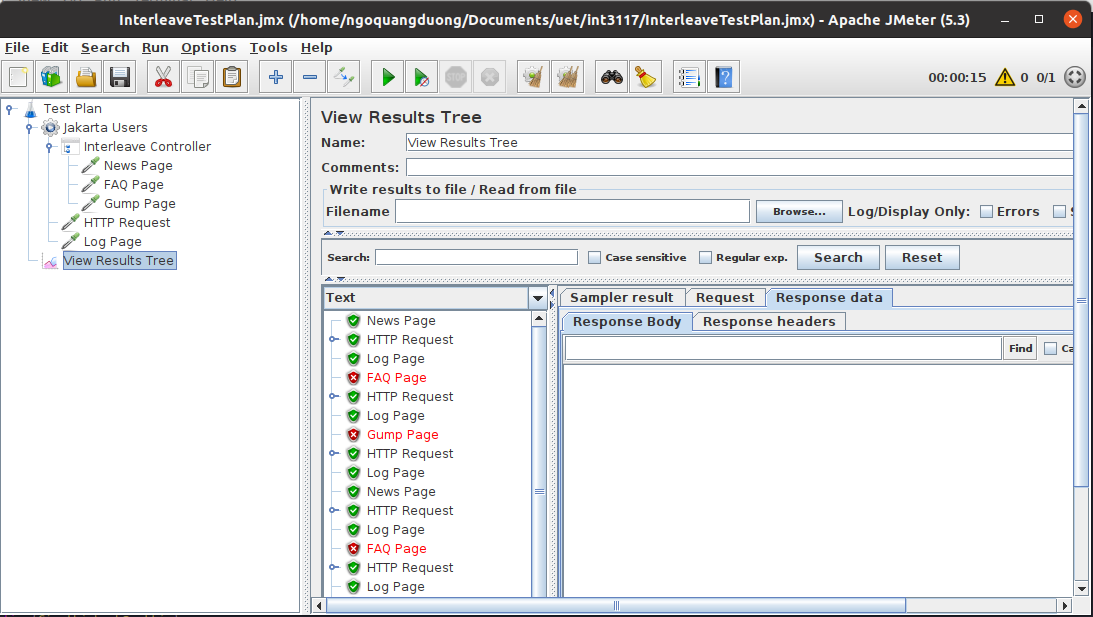
\includegraphics[scale=0.33]{interleave_controller.png}
              \caption{Ví dụ về Interleave Controller}
              {\label{fig:interleave-controller}}
          \end{figure}
          \FloatBarrier{}
          \par Trong hình~\ref{fig:interleave-controller}, \textbf{Interleave controller} chứa 3 samplers là \textit{News Page}, \textit{FAQ Page}, \textit{Gump Page}; cùng scope với \textbf{Interleave controller} là \textit{HTTP Request} và \textit{Log Page}. Thứ tự chạy của các sampler như sau:
          \begin{itemize}
              \item \textit{News Page}
              \item \textit{HTTP Request} và \textit{FAQ Page}
              \item \textit{FAQ Page}
              \item \textit{HTTP Request} và \textit{FAQ Page}
              \item \textit{Gump Page}
              \item \textit{HTTP Request} và \textit{FAQ Page}
              \item Lặp lại đến khi số lần lặp bằng giá trị đã cung cấp cho \texttt{loop count} của \textbf{Thread Group}.
          \end{itemize}
    \item \textbf{Switch controller}
          \par \textbf{Switch controller} gần giống với \textbf{Interleave controller}. Điểm khác biệt là \textbf{Switch controller} có thể nhận một thuộc tính \texttt{switch value} $-$ đây là index/tên của thành phần trong controller và thay vì chạy tuần tự các thành phần, \textbf{Switch controller} chỉ chạy thành phần khớp với \texttt{switch value}. Theo dõi thứ tự các request trong hình minh họa~\ref{fig:switch-controller}.
          \begin{figure}[htp]
              \centering
              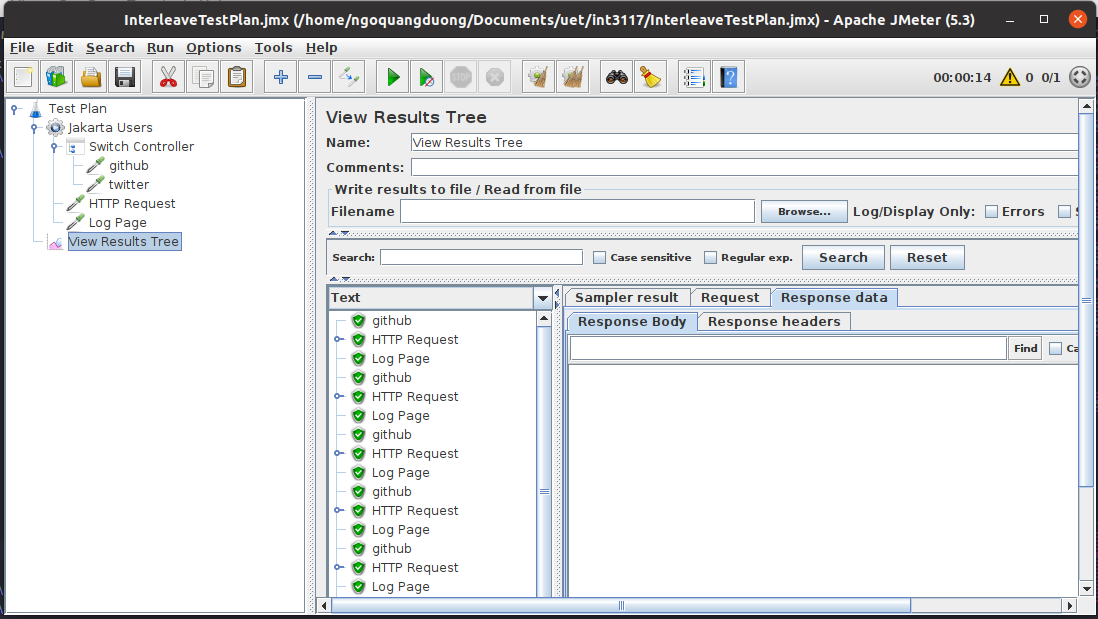
\includegraphics[scale=0.33]{switch_controller.png}
              \caption{Ví dụ về Switch controller}
              {\label{fig:switch-controller}}
          \end{figure}
    \item \textbf{Include controller}
          \par \textbf{Include controller} được tạo ra để \textbf{test plan} có thể sử dụng file \texttt{*.jmx} khác.
\end{itemize}

\section{Listener}

\par Nhiệm vụ của hầu hết các \textbf{Listener} trong một \textbf{test plan} là \textit{chờ} và \textit{lắng nghe} kết quả test. Như vậy, \textbf{Listener} sẽ thực hiện nhiệm vụ của mình sau khi các đối tượng cùng scope với nó đã chạy xong.

\par \textbf{Listener} thường được sử dụng cho các mục đích sau:

\begin{itemize}
    \item Xem request và response của các sampler (View Results Tree)
    \item Ghi lại kết quả ra một file (Simple Data Writer)
    \item Lưu response vào một file (Save Responses to a file)
    \item Hiển thị kết quả dạng bảng (View Results in Table)
    \item Tạo báo cáo dưới dạng bảng (Aggregate Report, Summary Report)
    \item Hiển thị kết quả, báo cáo dưới dạng biểu đồ (Aggregate Graph, Response Time Graph)
\end{itemize}

\section{Assertion}

\par \textbf{Assertion} là một trong những tính năng mà các công cụ kiểm thử mang lại, trong đó có cả \jmeter{}. \textbf{Assertion} được sử dụng để kiểm tra các samplers. Tuy nhiên, nếu trong một scope có một \textbf{Assertion} thì \textbf{Assertion} này sẽ thực hiện kiểm tra cho tất cả các samplers trong scope đó. Để \textbf{Assertion} chỉ kiểm tra cho một sampler cụ thể, cần phải đặt \textbf{Assertion} vào làm thành phần con của sampler đó.

\par \jmeter{} cung cấp nhiều loại \textbf{Assertion} khác nhau. Dưới đây là một số \textbf{Assertion} tiêu biểu.

\begin{itemize}
    \item \textbf{Response Assertion}: Kiểm tra response của một sampler. Có 4 kiểu kiểm tra: \texttt{Contains} và \texttt{Matches} sử dụng regex, \texttt{Equals} và \texttt{Substring} sử dụng plain text.
    \item \textbf{Duration Assertion}: Kiểm tra response có được trả về trong một thời lượng cho trước không (đo bằng millisecond).
    \item \textbf{Size Assertion}: Kiểm tra kích thước của response (có đủ 6 toán tử so sánh để lựa chọn)
    \item \textbf{XML Assertion}: Kiểm tra response có phải một tài liệu XML không (tuy nhiên không thể kiểm tra tài liệu XML đó có hợp lệ dựa trên DTD hay schema nào không).
    \item \textbf{BeanShell Assertion}: Cho phép thực hiện kiểm tra bằng BeanShell script (khác với các \textbf{Assertion} khác chỉ cần khai báo).
    \item \textbf{MD5Hex Assertion}: Kiểm tra MD5 hash của response.
    \item \textbf{HTML Assertion}: Kiểm tra cú pháp HTML của response.
    \item \textbf{XPath, XPath2 Assertion}: Kiểm tra thành phần một tài liệu XML bằng truy vấn XPath.
    \item \textbf{XML Schema Assertion}: Kiểm tra một tài liệu XML có hợp lệ đối với một XML schema hay không.
    \item \textbf{JSON Assertion}: Kiểm tra tài liệu JSON có hợp lệ không và kiểm tra JSON path.
\end{itemize}

\section{Timer}

\par Trong cùng một scope, \textbf{Timer} là thành phần chạy đầu tiên. \textbf{Timer} phải đi cùng với một sampler (cùng scope hoặc nằm trong sampler đó).

\par \textbf{Timer} pause thread trong một khoảng thời gian (do người dùng đưa ra) giữa các requests.

\section{Các thành phần khác}

\subsection{Tiền xử lý}

\par Thành phần tiền xử lý được sử dụng để sửa đổi sampler trong một scope. Dưới đây là một số thành phần tiền xử lý tiêu biểu

\begin{itemize}
    \item \textbf{HTML Link Parser}: Sau khi một sampler nhận được response data (ở dạng HTML), thành phần này sẽ phân tích tài liệu HTML đó và trích xuất ra các siêu liên kết và form. Sampler liền sau có thể sử dụng lại những giá trị được trích xuất này.
    \item \textbf{User Parameters}: Thành phần này cho phép tạo các biến cho từng user/thread.
    \item \textbf{Sample Timeout}: Thành phần này hẹn giờ để ngắt một sampler nếu sampler đó mất quá nhiều thời gian để hoàn thành.
\end{itemize}

\subsection{Hậu xử lý}

\par Thành phần hậu xử lý được thực thi sau các samplers, nhưng chạy trước các \textbf{Assertion}.

\par Đa số các thành phần hậu xử lý được cung cấp bởi \jmeter{} là các extractor $-$ chúng trích xuất các giá trị từ response của sampler.

\begin{itemize}
    \item \textbf{Regular Expression Extractor}: Trích xuất các giá trị từ response bằng regex (Perl regex).
    \item \textbf{CSS Selector Extractor}: Nếu response là một tài liệu HTML, thành phần này có thể trích xuất nội dung của các tag, các attribute bằng CSS selector.
    \item \textbf{XPath/XPath2 Extractor}: Nếu response là một tài liệu XML, thanh phần này có thể sử dụng truy vấn XPath/XPath 2.0 để trích xuất giá trị (có thể trích xuất nhiều giá trị cùng lúc).
    \item \textbf{JSON JMESPath Extractor}: Mặc dù có tên gọi như vậy nhưng thành phần này lại chỉ trích xuất giá trị từ tài liệu XML hoặc HTML. Tuy nhiên, mỗi lần chỉ có thể trích xuất được một giá trị.
    \item \textbf{JSON Extractor}: Thành phần này cho phép trích xuất dữ liệu là JSON response bằng JSON Path.
    \item \textbf{Boundary Extractor}: Thành phần này cho pehsp trích xuất các giá trị từ response thông qua việc cung cấp delimiter trái và phải.
\end{itemize}

\par Bên cạnh đó là các thành phân hậu xử lý khác.

\begin{itemize}
    \item \textbf{Result Status Action Handler}: Thành phần này cho phép đưa ra quyết định làm gì khi một sampler bị lỗi (dừng test hay chỉ dừng thread).
    \item \textbf{BeanShell/JSR223 PostProcessor}: Thành phần này cho phép một đoạn script BeanShell/JSR223 thực thi sau khi sampler thực hiện xong.
    \item \textbf{JDBC PostProcessor}: Thành phần này cho phép chạy các câu lệnh SQL sau khi sampler thực hiện xong $-$ điều này hữu ích khi muốn khôi phục cơ sở dữ liệu về trạng thái cũ sau khi JDBC sample thay đổi cơ sở dữ liệu.
\end{itemize}

\subsection{Cấu hình}

\par Các thành phần cấu hình được sử dụng để set up các giá trị mặc định và các biến để sau đó các samplers sử dụng. Do đó, chúng luôn được xử lý ở phần mở đầu của một scope, nói cách khác là trước mọi sampler trong scope đó.

\par Cấu hình trong \jmeter{} có thể là:
\begin{itemize}
    \item Các giá trị, các biến (CSV Data Set Config, User variable, Counter, Random variable).
    \item Request mặc định (FTP request, HTTP request, Java request, LDAP request, TCP sampler config).
    \item Cấu hình kết nối (JDBC connection, Bolt connection).
    \item Các trình quản lý dành cho giao thức HTTP (HTTP cache, HTTP cookie, HTTP header, HTTP authorization).
\end{itemize}

\section{Cách hoạt động}

\par Như vậy, chúng ta đã đi qua việc dùng thử \jmeter{} và mô tả khái quát các thành phần chính của một \textbf{Test Plan}. Tổng kết lại, khi một \textbf{Test Plan} chạy, trình tự xử lý của các thành phần là như sau:

\begin{itemize}
    \item Bắt đầu Thread
    \item Các cấu hình
    \item Logic Controller/Sampler
          \begin{itemize}
              \item Tiền xử lý
              \item Timer
              \item Logic Controller/Sampler con
              \item Assertion
              \item Listener
              \item Hậu xử lý
          \end{itemize}
    \item Lưu và hiển thị kết quả
    \item Lặp lại Thread
\end{itemize}

\end{document}
